% \section{openHAB}
% \label{sec:openhab} 
%     Neben der so eben erläuterten Home Assistant Plattform zählt ebenso die openHAB Plattform als bekannt und 
%     in der Anwendung populär. Der \ac{OPENHAB} ist eine Plattform, bei der es sich um eine 
%     Softwarelösung handelt, die auf Basis der Programmiersprache Java aufgebaut ist. Die Software steht unter 
%     der Eclipse Public License und fällt daher unter die Rubrik der Open-Source Software. Durch die Verwendung 
%     von Java ist die Anwendung betriebssystemunabhängig und kann auf beliebigen Betriebssystemen laufen. 
%     Ähnlich zu der vorgestellten Home Assistant Software, bietet openHAB ebenso User Interfaces die durch 
%     den Webbrowser, Android- und iOS-Geräte unterstützt werden. 
%     \\
%     \linebreak
%     In Kombination mit Java wird bei openHAB das \ac{OSGI}-Framework für die Modularität der Software verwendet. Mit Apache 
%     Karaf wird ein Container bereitgestellt, der mit Eclipse Equinox als \acs{OSGI} Laufzeitumgebung agiert. Als 
%     \acs{HTTP}-Server ist Jetty in Gebrauch. Die einzelnen Frameworks werden nicht im Detail erläutert, lediglich die für das 
%     Verständnis des Konzeptes notwendigen.
%     \\
%     \linebreak
%     Mit openHAB wird eine hochmodulare Software zur Verfügung gestellt, die durch sogenannte \textit{Add-ons} erweitert 
%     werden kann. Durch diese wird der Plattform eine breite Palette an Funktionen geboten. Physische Geräte können in 
%     großer Anzahl mit der Plattform interagieren und verknüpft werden.\footnote{Einleitung zu openHAB. \url{https://www.openhab.org/docs/} Abgerufen am 25.04.2022}

%     \subsection*{Historie}
%     \label{sec:historyoHAB}
%     Das Smart Home Projekt begann im November 2009 und wurde von Kai Kreuzer entwickelt\footnote{Chronologie und Blogbeiträge von Kai Kreutzer. \url{http://kaikreuzer.blogspot.com} Abgerufen am 28.04.2022.}. 
%     Im Februar 2010 wurde das Projekt unter dem Name openHAB bekannt. Nach zweieinhalb jähriger Entwicklung, im Dezember 2012, 
%     gab Herrn Kreutzer ein Statement zu der Verwendung von OSGi ab, die seine Überzeugung der Verwendung des Frameworks nach wie 
%     vor kundtut.
%     \begin{quote}
%         „Looking back at this evolution of the project, I am perfectly sure that if I had designed openHAB as a normal Java 
%         application instead of an OSGi application, it would not have prospered as it did. It is really the choice of the 
%         software architecture that made it happen - and as a nice side effect, the community is not a pure user community 
%         as it is the case for many other Open Source projects, but it is full of engaged people who actively contribute to the 
%         project.\cite{kaikreutzer2012}“
%     \end{quote} 
\subsubsection*{}
Mit der stetig wachsenden Anwendung und deren Community nimmt die Entwicklung des Projekts immer mehr Fahrt auf. 2014 betitelt 
Kreutzer das Jahr als Jahr des Smart Home, da die Beteiligung, das Interesse und die Entwicklung enorm zunahm und die Community immer 
großer wurde \cite{kaikreutzer2014}. Seitdem kamen weitere Unterstützungen zu anderen Geräten und 
Kommunikationsprotokollen dazu. Im Laufe der Entwicklung wurde eine mobile Anwendung entwickelt, mit der die Remotesteuerung 
implementiert ist. Die Software wird regelmäßig gepatched und von der Community unterstützt.

\subsection{Konzept und Architektur}
    Die Steuerungsplattform openHAB bietet vergleichbar zu Home Assistant die Möglichkeit der multifunktionalen Verknüpfung von 
    Geräten und Protokollen. An dieser Stelle werden ebenso mehrere Konzepte verwendet, die die Vereinheitlichung der Plattform 
    verstärkt. Die Konzepte der openHab Software sind in drei größere Rubriken aufgeteilt, die sich wie folgt zusammensetzen:
    \\
    \linebreak
    Die erste Rubrik sind die Dinge (Things), diese sind die Entitäten, die als physische Komponente zu einem System hinzugefügt 
    und viele Funktionalitäten als eines bereitstellen kann. Hierbei ist zu berücksichtigen, dass die sogenannten Dinge nicht 
    immer Geräte sein müssen, diese können auch andere überschaubare Informationsquellen, andere Webdienste und Funktionalitäten 
    darstellen. Aus Sicht des Benutzers sind sie für den Einrichtungs- und Konfigurationsprozess relevant, für den Betrieb 
    jedoch potentiell zu vernachlässigen. Dinge können Konfigurationseigenschaften haben, die optional oder obligatorisch sein 
    können. Solche Eigenschaften können grundlegende Informationen wie eine IP-Adresse, ein Zugriffstoken für einen Webdienst 
    oder eine gerätespezifische Konfiguration sein, die sein Verhalten ändert \cite{openHAB-article}. Mit dem Konzept der Dinge 
    kommen zwei Unterkategorien einher:
    \begin{itemize}
        \item Kanäle (Channels): Jedes Gerät, bzw. Ding stellt Kanäle bereit, mit denen die jeweiligen Funktionen abgebildet werden. 
        An der Stelle an der das physische Gerät angebunden ist, ist der Kanal eine konkrete Funktion dieser Entität. Beispielsweise 
        kann eine Glühbirne einen Kanal für die Farbtemperatur und einen für den Farbwert besitzen. Diese stellen beide die 
        Funktionalität der einen physischen Glühbirne für das System bereit. Grundlegend sind Kanäle mit Elementen verknüpft, mit denen 
        die virtuelle und physische Ebene verbunden wird. Ab dem Zeitpunkt, sobald eine Verbindung hergestellt wird, reagiert ein Ding 
        auf Ereignisse, die für ein Element transferiert werden. Bedingung dafür ist die Verknüpfung zu einem Kanal. Auf der anderen 
        Seite werden aktiv Ereignisse für Objekte gesendet, die mit Kanälen des Dings verknüpft sind \cite{openHAB-article}.
        \item Brücken (Bridges): Die Brücke ist eine besondere Art von Ding. Diese müssen dem System hinzugefügt werden, damit der 
        Zugriff auf andere Dinge ermöglicht wird, bzw. erhalten bleibt. Ein IP-Gateway für Hausautomationssysteme, welches nicht 
        IP-basiert funktioniert, ist eine typisches Beispiel für so eine Brücke.
    \end{itemize}
    An zweiter Stelle stehen die Artikel (Items). Diese Elemente stellen Funktionen dar, die direkt von der Anwendung verwendet 
    werden. Darunter zählen hauptsächlich die Automatisierungslogik oder auch Benutzeroberflächen. Durch Ereignisse werden die 
    Elemente verwendet, da diese einen Zustand besitzen. 
    \\
    Elemente können auch in eine Gruppe zusammengefasst werden. Ein Gruppenelement kann auch Mitglied einer weiteren Gruppe sein. 
    Diese zyklischen Mitgliedschaften sind war nicht verboten, davon wird jedoch abgeraten. Über Benutzeroberflächen können 
    einzelne Gruppenelemente als alleinstehender Eintrag angezeigt werden und eine Navigation zu den jeweiligen Mitgliedern 
    bereitstellen. 
    \\
    \linebreak
    Die dritte große Rubrik sind die Bindungen und Links (Bindings and Links). Diese können als Softwareadapter betrachtet werden, 
    die Dinge für ihr Hausautomationssystem zur Verfügung stellen \cite{openHAB-article}. Aufgabe der Komponente ist die Verknüpfung 
    von Elementen mit physischen Geräten. Um dies zu ermöglichen werden die spezifischen Kommunikationsanforderungen eines Geräts 
    abstrahiert. Dadurch ist eine allgemeinere Behandlung der Komponente durch das Framework möglich. Links stellen das Bindeglied 
    zwischen Dingen und Gegenständen dar. Es ist die Verknüpfung von genau einem Element und einem Kanal. Elemente und 
    Kanäle haben keine eins zu eins Beziehung zueinander. Eine Verknüpfung mit mehreren Komponenten ist auch hier möglich. 
    \\
    \linebreak
    Neben den übergreifenden Konzepten gibt es weitere Konzepte\footnote{Historie und Konzepte von openHAB. \url{https://medium.com/smartsmarthome/openhab-41c30d50fc42} Abgerufen am 28.04.2022}. 
    Diese werden in Folgendem aufgelistet:
    \begin{itemize}
        \item Seitenverzeichnis (Sitemaps): Dies beinhaltet die Konfiguration eines Seitenverzeichnisses, mit dem Schalter, 
        Regler, Texte und vieles mehr hinzugefügt werden kann. Diese Ansichten repräsentieren den Status eines Elements und 
        können darüber gesteuert und überprüft werden.
        \item Regeln (Rules): Eine Regel ist die Verknüpfung eines Ereignisses und einer Aktion. Somit wird nach einem bestimmten 
        Ereignis eine Aktion ausgeführt. Ein Beispiel: Wenn ein Fenster geöffnet wird, soll die Heizung abgeschaltet werden. 
        So lange, bis das Fenster wieder geschlossen wird. 
        \item Persistenz (Persistence): Mit der Persistenzschicht kann festgelegt werden, welche historischen Zustandsereignisse 
        und Informationen gespeichert werden sollen. Dadurch kann nach Systemausfall der Status des Elementes wiederhergestellt werden. 
        \item Modelle (Models): Modelle stellen baumbasierte Gruppierungen von Elementen dar. In der Baumstruktur können Elemente 
        Orte, Punkte und Ausrüstungen sein. Ein Beispiel: Das Wohnzimmer als Standort besteht aus zwei Geräten Heizung und Licht. 
        Die Heizung als Ausstattung hat zwei Punkte: \textit{Ist-Temperatur} und \textit{Soll-Temperatur}.
        \item Seiten (Pages):Alle Seiten und Seitenverzeichnisse kontrollieren die Zustände von Elementen und greifen auf diese zu. 
        Mit openHAB 3 würden weitere Möglichkeiten hinzugefügt, um benutzerdefinierte \acs{UI}, Diagramme, Grundrisse und oder 
        Layouts zu definieren. 
        \item Skripte (Scripts): Skripte sind ähnlich zu den Regeln. Diese spezifizieren eine Aktion und kein Ereignis. Die Skripte 
        können manuell, aber auch über andere Skripte und Regeln ausgeführt werden. 
    \end{itemize}
    Die anfängliche Architektur der openHAB Anwendung teilt sich in drei Sektionen auf: Die Kernkomponenten (blau), das drunter 
    liegende OSGi-Framework (grün) und die Erweiterungen (Add-Ons) (gelb). 
    \begin{figure}[hbt!]
        \centering
        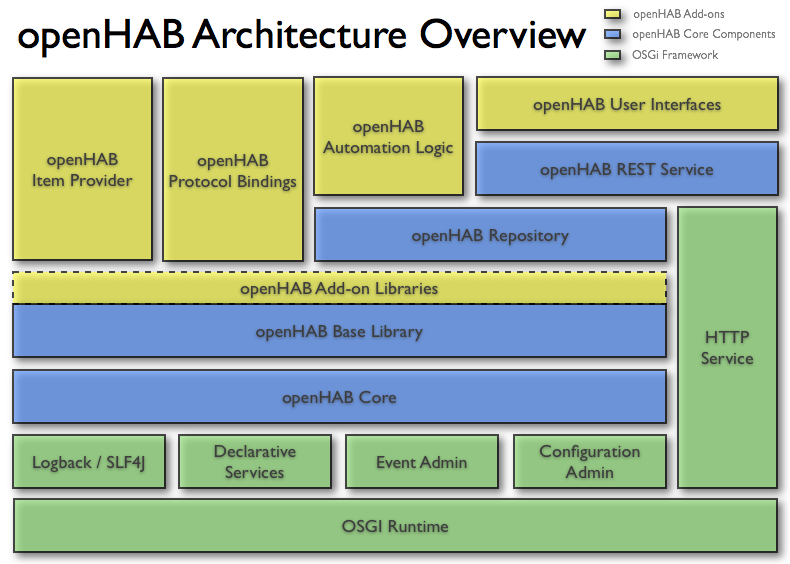
\includegraphics[width=15cm,height=15cm,keepaspectratio]{images/openhab-architecture.png}
        \caption{Architektur der openHAB Plattform \cite{openHAB-architecture2013}}
        \label{fig:architectureopenHAB}
    \end{figure}
    \\
    %\pagebreak
    \linebreak
    Mit der wesentlichen Aktualisierung von openHAB zur aktuellen Version openHAB 2.0 gab es auch einige Änderungen an der 
    grundlegenden Architektur. Es basiert hauptsächlich auf dem Eclipse SmartHome Framework und nutzt Apache Karaf zusammen mit 
    Eclipse Equinox, um eine \acs{OSGI} Laufzeitumgebung zu erstellen. Jetty wird als \acs{HTTP} Server verwendet. 
    \\
    \linebreak
    \textit{Eclipse SmartHome}\footnote{Eclipse SmartHome. \url{https://projects.eclipse.org/projects/iot.smarthome} Abgerufen am 29.04.2022} 
    ist ein \acs{IoT} Projekt, welches sich aus der ersten Version der openHAB Plattform entwickelte. 
    Diese wurde von der Eclipse Foundation übernommen und weiterentwickelt. Es stellt das Kern-Framework für Smart Home Systeme dar 
    und ist essentieller Bestandteil der openHAB Plattform. Das Framework ist mittlerweile archiviert und erhält keine weiteren 
    Aktualisierungen.
    \\
    \linebreak
    \textit{Apache Karaf}\footnote{Apache Karaf. \url{https://karaf.apache.org/} Abgerufen am 29.04.2022} 
    ist eine \acs{OSGI} basierte Laufzeitumgebung über die verschiedene Komponenten mittels Container 
    bereitgestellt werden können. Dieses Framework zählt zu denen der Apache Software Foundation und unterliegt der Apache V2 Lizenz.
    \\
    \linebreak
    \textit{Eclipse Equinox}\footnote{Eclipse Equinox. \url{https://www.eclipse.org/equinox/} Abgerufen am 29.04.2022} ist eine modulare 
    Java basierte Laufzeitumgebung und eine Implementierung des \acs{OSGI} Framework. Der Begriff der \textit{Bundles} ist das 
    Herzstück der \acs{OSGI}-Spezifikation. Diese werden verwendet, damit die Modularität für Java erfasst wird. Ein Bundle ist 
    ein Standard-Java-JAR-Datei, dessen Manifest zusätzliches Markup enthält, welches das Bundle identifiziert und seine Abhängigkeiten 
    angibt. Als solches ist jedes Bundle vollständig selbstbeschreibend \cite{openHAB-article}. 
    \begin{figure}[hbt!]
        \centering
        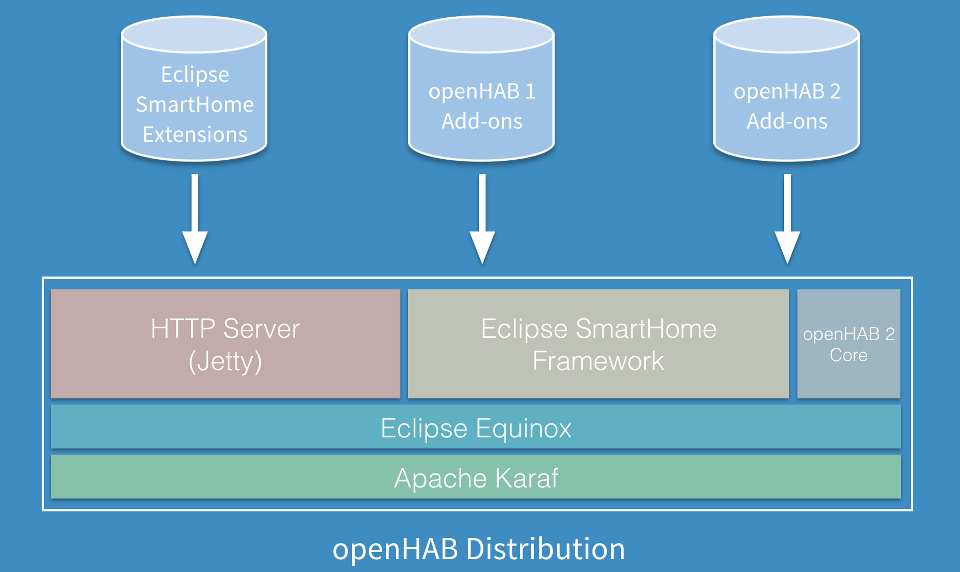
\includegraphics[width=15cm,height=15cm,keepaspectratio]{images/openhab-2-architecture.png}
        \caption{Architektur der openHAB 2.0 Plattform \cite{kaikreutzer2016}}
        \label{fig:architectureopenHAB2}
    \end{figure}
    \\
    \textit{OSGi} fördert den modularen Aufbau von Software, die mit der Programmiersprache Java geschrieben ist. Der Open-Source 
    Standard bietet einen Ansatz, der eine modulare Plattform beschreibt und eine \ac{JVM} voraussetzt. Die \acl{JVM}\footnote{Detaillierte Beschreibung der JVM. \url{https://www.javatpoint.com/jvm-java-virtual-machine} Abgerufen am 01.05.2022} 
    ist der Teil der Java-Laufzeitumgebung, die für die Ausführung des Java-Bytecodes verantwortlich ist.
    \\
    Die sogenannten \textit{Bundles} sind Module und bilden die kleinste Einheit der Modularisierung. Aus technischer Sicht ist 
    dieses Konstrukt eine \ac{JAR}-Datei mit Metainformationen. Diese sind in einer Manifestdatei gespeichert. Bundles sind 
    eindeutig zu identifizieren. Dadurch ist es in \acs{OSGI} möglich, \textit{Bundles} mit demselben Namen, jedoch unterschiedlicher 
    Versionen gleichzeitig zu nutzen und auszuführen \cite{openHAB-article}. 
    \begin{figure}[hbt!]
        \centering
        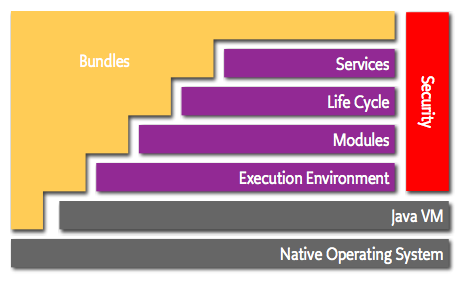
\includegraphics[width=10cm,height=10cm,keepaspectratio]{images/osgi-architecture.png}
        \caption{OSGi Schichtenarchitektur \cite{openhab-osgi}}
        \label{fig:osgilayer}
    \end{figure}
    \\
    %\linebreak
    Weitere Details der \acs{OSGI}-Architektur\footnote{Architektur und Erläuterung OSGi. \url{https://www.openhab.org/docs/developer/osgi/osgi.html} Abgerufen am 01.05.2022} 
    sind der openHAB Dokumentation zu entnehmen.

\subsection{Ziele und Schwerpunkte} 
    \begin{quote}
        „openHAB empowering the smart home\footnote{Log und Label von openHAB \url{https://www.openhab.org/} Abgerufen am 01.05.2022}“
    \end{quote}
    Das große Ziel, dass mit der openHAB Anwendung verfolgt wird, ist allgemein die zentrale Steuerung von Geräten innerhalb eines 
    Wohnraumes.
    \begin{quote}
        „... is an open source, technology agnostic home automation platform which runs as the center of your smart home!\footnote{Einleitung und Übersicht der openHAB Dokumentation. \url{https://www.openhab.org/docs/} Abgerufen am 01.05.2022}“
    \end{quote}
    
\subsection{Stärken und Schwächen}
    Die Stärken, die openHAB mit sich bringt, werden schon in den Dokumentationen aufgegriffen und bei der Nutzung der Anwendung 
    schnell deutlich. Mit der Plattform können eine Vielzahl von Geräten und Systemen integriert werden, die miteinander 
    kommunizieren. In der einzigen von openHab gegebenen Lösung können Heimautomatisierungssysteme, intelligente Geräte und 
    andere Technologien, darunter beispielsweise Kommunikationsprotokolle, integriert werden \cite{openhab-strength}. Durch die in 
    dem letzten großen Update der Plattform hinzukommende einheitliche Benutzeroberfläche, die die Bedienung von Geräten und 
    Systemen vereinfacht, ist die Integration von neuen Geräten einfacher. Mit dem Ansatz von 
    Automatisierungsregeln können alle Geräte bei Bedarf miteinander Kommunizieren. Das Aufstellen von solchen Regeln ist 
    herstellerunabhängig und macht die Automatisierung flexibler. Der dritte und letzte Punkt der Stärken ist die allgemeine 
    Vielfältigkeit und Flexibilität der Plattform. Hiermit ist im Allgemeinen die Umsetzung von Use Cases und Automatisierungen 
    gemeint. Dem Nutzer sind keine Grenzen der Kompatibilität gesetzt.
    \\
    \linebreak
    Im Gegenzug sind die Schwächen hauptsächlich Auswirkungen der komplexen und weitgestrickten Architektur. Das System an sich 
    und der Umgang damit stellt sich als komplex dar. In das Aufsetzen und Verstehen der Plattform, deren Konzepte und 
    Möglichkeiten muss ein hoher Aufwand gesteckt werden. Die Dokumentation der Software geht auf diese Aspekte ein und gibt dem 
    Leser mit, dass die Software nicht innerhalb kürzester Zeit verstanden werden kann \cite{openhab-strength}. 
    \\
    Eine weitere größere Schwäche ist die Weiterentwicklung des Systems. Diese findet langsam und nicht konstant statt. Auslöser 
    dafür ist die Architektur und deren Abhängigkeiten zu weiteren Frameworks und Bibliotheken. Auch nimmt der Prozess bis zur 
    Genehmigung von Weiterentwicklungen viel Zeit in Anspruch. Dies ist möglicherweise mit ein Grund, weshalb neue Versionen und 
    Updates nur unregelmäßig zu beobachten sind. 

\section{Vergleich von Home Assistant und openHAB}
\label{sec:comparison-HAOS-openHAB}
    %Allgemein gültiger Vergleich (Aufbau, Architektur, Schwerpunkte (Fokus), Umsetzungen, Konnektivität, etc.)
    % https://everythingsmarthome.co.uk/home-assistant-vs-openhab-which-one-is-better/
    % https://smarthome.msuttner.de/openhab-2/vergleich-openhab-vs-home-assistant/ 
    % https://www.electronicshub.org/openhab-vs-home-assistant/ 
    % https://smarthome.university/your-smart-home-platform-home-assistant-vs-openhab/ 
    % https://purdylounge.com/openhab-vs-home-assistant/ 
    Nach der Erläuterung der beiden Softwarelösungen im Bereich der Smart Home Plattformen, werden diese abschließend 
    gegenübergestellt, um weiter Aspekte miteinander zu vergleichen. Grundlage dafür sind persönliche Erfahrungen als auch 
    Erfahrungen und Eindrücke von Nutzern und Experten. Die Tabelle (\ref{tab:comparisonTableHAOS-openHAB}) zum Vergleich 
    der Plattformen ist dem Anhang ... zu entnehmen.
    \\
    Zusammenfassend zu dieser tabellarischen Gegenüberstellung ist zu sagen, dass beide Plattformen ihre markanten Stärken vorweisen. 
    Beide Ansätze bieten eine gute Grundlage, die Automatisierungen in dem eigenen Gebäude voranzutreiben. Die Entscheidung, welches 
    Tool verwendet werden soll, liegt in der Verantwortung des Nutzers. Übergreifend sind die beiden Open-Source Lösungen eine gute 
    Alternative zu kommerziellen Produkten und Lösungen, sofern der Nutzer herstellerunabhängig interagieren möchte.
    \begin{table}[hbt!]
        \begin{center}
            \begin{tabular}{| p{3.15cm} | p{6.3cm} | p{6.3cm} | }
                \hline
                   \textbf{Attribut} & \textbf{openHAB} & \textbf{Home Assistant} \\
                \hline
                    Architektur & Robustheit und Starrheit, sowie die gewissenhafte Entwicklung & Erfordert häufigere Updates, bietet jedoch eine schnelle Entwicklung und eine viel modernere und anspruchsvollere Architektur \cite{sh-uni-comparison}. \\ 
                \hline
%                    Installation und Wartung & Installation ist genauestens dokumentiert. Initiale Konfiguration muss über die Kommandozeile durchgeführt werden, Updates ebenso. & Ein-Klick-Installationsprozess. Initiale Konfiguration benötigt das Verständnis von YAML-Dateien. Updates können über die UI verwaltet werden \cite{sh-uni-comparison}. \\ 
%                \hline
%                    Unterstützte Geräte und Verknüpfungen & Durch die gängigen Smart Home Protokolle werden über 1000 Komponenten unterstützt. & Home Assistant unterstützt ebenso über 1000 Komponenten, wobei die Benutzerfreundlichkeit beim Anlegen und Verwalten bei Home Assistant deutlich angenehmer und leichter erscheint \cite{msuttner-comparison}. \\ 
%                \hline
%                    Automatisierungsregeln & Bereitstellung von Automationen durch Xtend. Xtend ist ein flexibler und ausdrucksstarker Java-Dialekt, der sich in Quellcode basierend auf Java 8 kompilieren lässt. Ebenso können über Blockly Automatisierungsregeln erstellt werden. Blocky ist eine clientseitige JavaScript Bibliothek, die visuelle Blöcke mit Anweisungen, Bedingungen uvm. erstellen und editieren lässt. Eine weitere Alternative ist die Verwendung von Node-RED.  & Home Assistant bietet die Möglichkeit, Automatisierungen per YAML zu erstellen. Alternativ mit Node-RED. YAML-Dateien sind flexibler, jedoch nicht unbedingt benutzerfreundlich. \\ 
%                \hline
%                    User Interface & openHAb hat in den User Interface viele Duplikate und zu viele ähnliche Optionen zur Verfügung bei unterschiedlicher Oberfläche. & Die Benutzeroberfläche der Home Assistant Plattform ist für Einsteiger und Anfänger deutlich benutzerfreundlicher und weniger komplex als openHAB. \\
%                \hline
%                    Mobile Anwendungen & openHAB bietet eine dedizierte App für iOS und Android. Diese ist mit innovativen Optionen ausgestattet.  & Home Assistant bietet ebenso eine App für iOS und Android, jedoch bei weitem nicht so stark entwickelt als die von openHAB. Die Benachrichtigungsdienste sind jedoch mit Home Assistant besser genutzt. \\ 
%                \hline
%                    Community und Dokumentation & openHAB bietet eine sehr starke und repräsentative Community. Die Dokumentation ist ausführlich und beschreibt die Prozesse, Konzept und Architektur ausführlich. & Home Assistant unterscheidet sich in diesen Punkten nicht von openHAB. Eine starke Community und eine solide Dokumentation der Plattform.  \\
%                \hline
%                    Vergleich von Xtend \& YAML &  &  \\ 
%                \hline 
            \end{tabular}
        \end{center}
        \caption{Vergleich der Plattformen \cite{sh-uni-comparison} \cite{msuttner-comparison} \cite{barclay-comparison}}
        \label{tab:comparisonTableHAOS-openHAB}
    \end{table}

 